\documentclass[12pt,a4paper]{article}
\usepackage[utf8]{inputenc}
\usepackage[T1]{fontenc}
\usepackage[margin=0.8in]{geometry}
\usepackage{graphicx}
\usepackage[hidelinks]{hyperref}
\usepackage{listings}
\usepackage{xcolor}
\usepackage{tikz}
\usepackage{booktabs}
\usepackage{longtable}
\usepackage{float}
\usepackage{fancyhdr}
\usepackage{tcolorbox}
\usepackage{fontawesome5}
\usetikzlibrary{shapes,arrows.meta,positioning,shadows}

% Colors
\definecolor{primaryblue}{RGB}{26,82,118}
\definecolor{accentgreen}{RGB}{39,174,96}
\definecolor{warnorange}{RGB}{243,156,18}
\definecolor{codebg}{RGB}{248,249,250}
\definecolor{codeframe}{RGB}{200,200,200}

% Code styling
\lstset{
    backgroundcolor=\color{codebg},
    frame=single,
    rulecolor=\color{codeframe},
    basicstyle=\ttfamily\small,
    breaklines=true,
    commentstyle=\color{gray},
    keywordstyle=\color{primaryblue}\bfseries,
    stringstyle=\color{accentgreen}
}

% Header/Footer
\pagestyle{fancy}
\fancyhf{}
\fancyhead[L]{\textcolor{primaryblue}{\textbf{PKG2020 Viva Guide}}}
\fancyhead[R]{\textcolor{gray}{KRR Project}}
\fancyfoot[C]{\thepage}

% Custom boxes
\newtcolorbox{conceptbox}[1]{
    colback=primaryblue!5,
    colframe=primaryblue,
    title={\faLightbulb\ #1},
    fonttitle=\bfseries
}

\newtcolorbox{codebox}[1]{
    colback=codebg,
    colframe=codeframe,
    title={\faCode\ #1},
    fonttitle=\bfseries\ttfamily
}

\newtcolorbox{tipbox}{
    colback=accentgreen!10,
    colframe=accentgreen,
    title={\faCheckCircle\ Key Point},
    fonttitle=\bfseries
}

\newtcolorbox{warnbox}{
    colback=warnorange!10,
    colframe=warnorange,
    title={\faExclamationTriangle\ Important},
    fonttitle=\bfseries
}

\begin{document}

% ============== TITLE PAGE ==============
\begin{titlepage}
\centering
\vspace*{1cm}

{\Huge\textcolor{primaryblue}{\textbf{PKG2020 Knowledge Graph}}}\\[0.5cm]
{\LARGE\textcolor{gray}{Viva Preparation Guide}}\\[1cm]

\rule{\textwidth}{2pt}\\[0.5cm]
{\large Complete Walkthrough of Project Components}\\[0.5cm]
\rule{\textwidth}{2pt}\\[2cm]

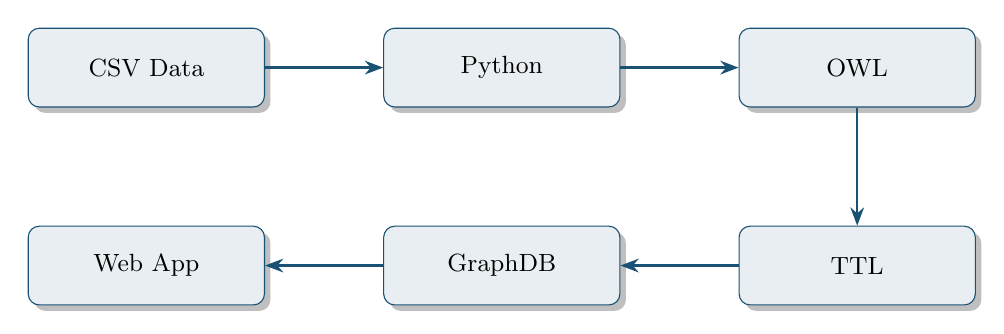
\begin{tikzpicture}[
    node distance=1.5cm,
    box/.style={rectangle, draw=primaryblue, fill=primaryblue!10, rounded corners, minimum width=3cm, minimum height=1cm, font=\small, drop shadow}
]
\node[box] (csv) {CSV Data};
\node[box, right=of csv] (python) {Python};
\node[box, right=of python] (owl) {OWL};
\node[box, below=of owl] (ttl) {TTL};
\node[box, left=of ttl] (graphdb) {GraphDB};
\node[box, left=of graphdb] (webapp) {Web App};

\draw[-{Stealth}, thick, primaryblue] (csv) -- (python);
\draw[-{Stealth}, thick, primaryblue] (python) -- (owl);
\draw[-{Stealth}, thick, primaryblue] (owl) -- (ttl);
\draw[-{Stealth}, thick, primaryblue] (ttl) -- (graphdb);
\draw[-{Stealth}, thick, primaryblue] (graphdb) -- (webapp);
\end{tikzpicture}

\vfill

{\Large\textbf{Project Statistics}}\\[0.5cm]
\begin{tabular}{|c|c|c|c|}
\hline
\textbf{23 Classes} & \textbf{14 Object Props} & \textbf{17+ Data Props} & \textbf{2.2M Triples} \\
\hline
\end{tabular}

\vfill
{\large Knowledge Representation and Reasoning}\\
{\large Fall 2025}
\end{titlepage}

% ============== TABLE OF CONTENTS ==============
\tableofcontents
\newpage

% ============== SECTION 1: PROJECT OVERVIEW ==============
\section{Project Overview}

\begin{conceptbox}{What is this Project?}
This project converts the \textbf{PKG2020S4 PubMed Knowledge Graph} dataset from flat CSV files into a semantic \textbf{OWL ontology} with linked data capabilities, published via a \textbf{SPARQL endpoint}.
\end{conceptbox}

\subsection{Domain: Biomedical Research Data}

The dataset contains:
\begin{itemize}
    \item \textbf{Articles}: Research publications identified by PubMed IDs (PMIDs)
    \item \textbf{Authors}: Researchers identified by AND\_IDs
    \item \textbf{Organizations}: Universities, research labs, hospitals
    \item \textbf{Career Data}: Employment and education history
    \item \textbf{BioEntities}: Genes, diseases, chemicals, mutations
    \item \textbf{NIH Funding}: Research project associations
\end{itemize}

\subsection{Deployed URLs}

\begin{tabular}{|l|l|}
\hline
\textbf{Web Application} & \url{https://krr-685beba13d3f.herokuapp.com} \\
\hline
\textbf{GraphDB Endpoint} & \url{https://x1327f4041a654297998.sandbox.graphwise.ai} \\
\hline
\textbf{GitHub Repository} & \url{https://github.com/Zain-ul-abdeen-773/Knowlege-Graphs-Project} \\
\hline
\end{tabular}

% ============== SECTION 2: KEY CONCEPTS ==============
\newpage
\section{Key Concepts for Viva}

\subsection{T-Box vs A-Box}

\begin{conceptbox}{T-Box (Terminological Box)}
The \textbf{schema/vocabulary} - defines classes, properties, and axioms.
\begin{itemize}
    \item Classes: Article, Author, Gene, Disease
    \item Properties: writtenBy, hasAffiliation, mentionsBioEntity
    \item Axioms: ``Every Article has at least 1 Author''
\end{itemize}
\textbf{File}: \texttt{pkg2020\_tbox\_only.owl}
\end{conceptbox}

\begin{conceptbox}{A-Box (Assertion Box)}
The \textbf{instance data} - actual individuals and their relationships.
\begin{itemize}
    \item Article\_12345678 is an Article
    \item Article\_12345678 writtenBy Author\_ABC
    \item Author\_ABC hasAffiliation Affiliation\_XYZ
\end{itemize}
\textbf{File}: \texttt{pkg2020\_final.owl} (contains both T-Box + A-Box)
\end{conceptbox}

\subsection{Defined Classes}

\begin{tipbox}
A \textbf{defined class} has \textbf{necessary AND sufficient conditions}. The reasoner can automatically classify individuals into defined classes!
\end{tipbox}

\begin{tabular}{|l|l|l|}
\hline
\textbf{Class} & \textbf{Definition} & \textbf{Type} \\
\hline
ActiveAuthor & Author $\sqcap$ $\exists$careerStartYear.int & Intersection \\
AnonymousAuthor & Author $\sqcap$ $\neg$ActiveAuthor & Complement \\
ResearchEntity & Author $\sqcup$ Article & Union \\
ProlificAuthor & Author $\sqcap$ writtenBy.min(5) & Cardinality \\
\hline
\end{tabular}

\subsection{Property Types}

\begin{tabular}{|l|l|l|}
\hline
\textbf{Type} & \textbf{Example} & \textbf{Meaning} \\
\hline
Functional & hasPrimaryAuthor & Max 1 value \\
Inverse Functional & hasPMID & Unique identifier \\
Symmetric & sameAs & A→B means B→A \\
Transitive & hasPart & A→B→C means A→C \\
\hline
\end{tabular}

% ============== SECTION 3: PROJECT FILES ==============
\newpage
\section{Project Files Explained}

\subsection{Directory Structure}

\begin{lstlisting}[language=bash]
Project/
├── data/                    # CSV source files
│   ├── OA01_Author_List.csv      # Authors & articles
│   ├── OA02_Bio_entities_Main.csv # Genes, diseases
│   ├── OA03_Bio_entities_Mutation.csv
│   ├── OA04_Affiliations.csv     # Author affiliations
│   ├── OA05_Researcher_Employment.csv
│   ├── OA06_Researcher_Education.csv
│   └── OA07_NIH_Projects.csv     # NIH funding
├── owl/                     # Generated OWL files
│   ├── pkg2020_tbox_only.owl     # Schema only (T-Box)
│   ├── pkg2020_hand_annotated.owl # 10+ test individuals
│   ├── pkg2020_with_swrl.owl     # SWRL rules
│   ├── pkg2020_final.owl         # Complete ontology
│   └── pkg2020_final.ttl         # Turtle for GraphDB
├── scripts/                 # Python scripts
│   └── [16 Python files]
└── docs/                    # Documentation
\end{lstlisting}

\subsection{Python Scripts Pipeline}

\begin{center}
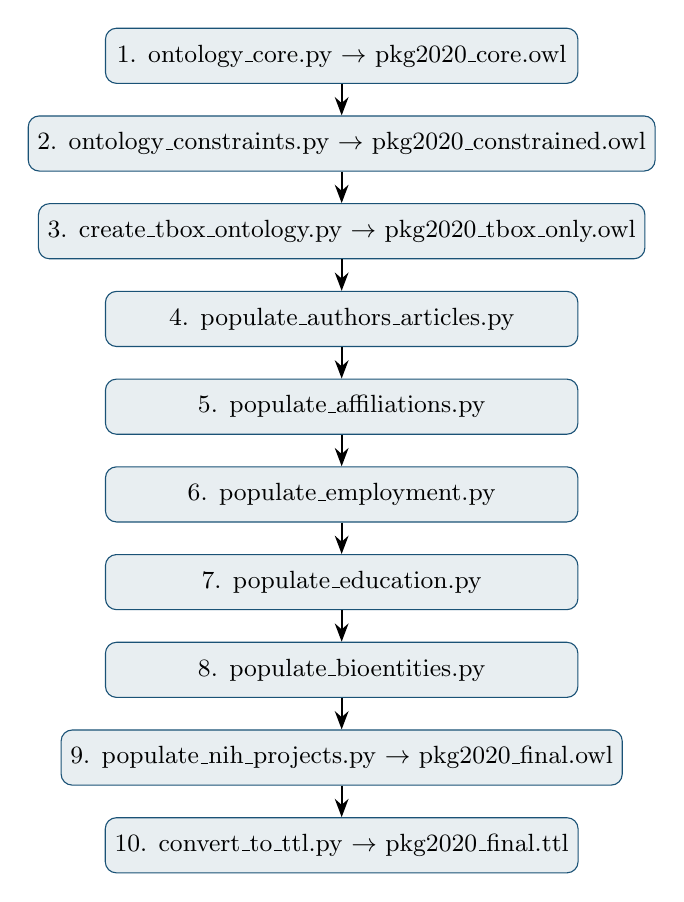
\begin{tikzpicture}[
    node distance=0.4cm,
    box/.style={rectangle, draw=primaryblue, fill=primaryblue!10, rounded corners, minimum width=6cm, minimum height=0.7cm, font=\small}
]
\node[box] (s1) {1. ontology\_core.py $\rightarrow$ pkg2020\_core.owl};
\node[box, below=of s1] (s2) {2. ontology\_constraints.py $\rightarrow$ pkg2020\_constrained.owl};
\node[box, below=of s2] (s3) {3. create\_tbox\_ontology.py $\rightarrow$ pkg2020\_tbox\_only.owl};
\node[box, below=of s3] (s4) {4. populate\_authors\_articles.py};
\node[box, below=of s4] (s5) {5. populate\_affiliations.py};
\node[box, below=of s5] (s6) {6. populate\_employment.py};
\node[box, below=of s6] (s7) {7. populate\_education.py};
\node[box, below=of s7] (s8) {8. populate\_bioentities.py};
\node[box, below=of s8] (s9) {9. populate\_nih\_projects.py $\rightarrow$ pkg2020\_final.owl};
\node[box, below=of s9] (s10) {10. convert\_to\_ttl.py $\rightarrow$ pkg2020\_final.ttl};

\draw[-{Stealth}, thick] (s1) -- (s2);
\draw[-{Stealth}, thick] (s2) -- (s3);
\draw[-{Stealth}, thick] (s3) -- (s4);
\draw[-{Stealth}, thick] (s4) -- (s5);
\draw[-{Stealth}, thick] (s5) -- (s6);
\draw[-{Stealth}, thick] (s6) -- (s7);
\draw[-{Stealth}, thick] (s7) -- (s8);
\draw[-{Stealth}, thick] (s8) -- (s9);
\draw[-{Stealth}, thick] (s9) -- (s10);
\end{tikzpicture}
\end{center}

% ============== SECTION 4: RUBRIC COMPLIANCE ==============
\newpage
\section{Rubric Compliance Checklist}

\subsection{Classes Requirements}

\begin{tabular}{|p{5cm}|p{3cm}|p{5cm}|}
\hline
\textbf{Requirement} & \textbf{Status} & \textbf{Location} \\
\hline
20+ classes & \checkmark\ 23 classes & create\_tbox\_ontology.py:16-107 \\
\hline
Enumeration class & \checkmark & ontology\_core.py:25-37 \\
& & \texttt{PublicationStatus = OneOf([...])} \\
\hline
Cardinality restrictions & \checkmark & ontology\_constraints.py:21-29 \\
& & \texttt{writtenBy.min(1, Author)} \\
\hline
Union class & \checkmark & ontology\_constraints.py:38-43 \\
& & \texttt{Author | Article} \\
\hline
Intersection class & \checkmark & ontology\_constraints.py:31-36 \\
& & \texttt{Author \& careerStartYear.some(int)} \\
\hline
Complement class & \checkmark & ontology\_constraints.py:45-50 \\
& & \texttt{Author \& Not(ActiveAuthor)} \\
\hline
\end{tabular}

\subsection{Properties Requirements}

\begin{tabular}{|p{5cm}|p{3cm}|p{5cm}|}
\hline
\textbf{Requirement} & \textbf{Status} & \textbf{Location} \\
\hline
7+ object properties & \checkmark\ 14 & create\_tbox\_ontology.py:110-181 \\
\hline
Functional property & \checkmark & ontology\_core.py:55-59 \\
& & \texttt{hasPrimaryAuthor} \\
\hline
Inverse functional & \checkmark & ontology\_constraints.py:17-19 \\
& & \texttt{hasPMID} \\
\hline
3+ range restrictions & \checkmark & Multiple files \\
\hline
7+ data properties & \checkmark\ 17+ & create\_tbox\_ontology.py:184-273 \\
\hline
\end{tabular}

% ============== SECTION 5: SPARQL QUERIES ==============
\newpage
\section{SPARQL Competency Queries}

\subsection{15 Competency Questions}

\begin{longtable}{|c|p{8cm}|p{3cm}|}
\hline
\textbf{\#} & \textbf{Question} & \textbf{Key Pattern} \\
\hline
CQ1 & Authors at multiple institutions & GROUP BY, HAVING \\
CQ2 & Most prolific authors & COUNT, ORDER BY \\
CQ3 & Author collaborations & Self-join on Article \\
CQ4 & Articles with genes & Class filter (pkg:Gene) \\
CQ5 & Articles with species & OPTIONAL \\
CQ6 & Gene-mutation correlations & Multiple FILTER \\
CQ7 & Bio-entity distribution & COUNT by type \\
CQ8 & Top organizations & COUNT affiliations \\
CQ9 & Affiliations by country & GROUP BY country \\
CQ10 & Top education institutions & COUNT education \\
CQ11 & Employment timeline & FILTER years \\
CQ12 & Authors with education & EXISTS \\
CQ13 & NIH funded authors & hasProject pattern \\
CQ14 & Principal investigators & piName property \\
CQ15 & Complete author profile & Multiple OPTIONAL \\
\hline
\end{longtable}

\subsection{Sample Query: CQ1}

\begin{codebox}{Authors at Multiple Institutions}
\begin{lstlisting}[language=SPARQL]
PREFIX pkg: <http://example.org/pkg2020/ontology.owl#>

SELECT ?author ?lastName (COUNT(DISTINCT ?org) AS ?count)
WHERE {
    ?author a pkg:Author .
    ?author pkg:lastName ?lastName .
    ?author pkg:hasAffiliation ?aff .
    ?aff pkg:affiliatedWith ?org .
}
GROUP BY ?author ?lastName
HAVING (COUNT(DISTINCT ?org) > 1)
ORDER BY DESC(?count)
LIMIT 20
\end{lstlisting}
\end{codebox}

% ============== SECTION 6: SWRL RULES ==============
\newpage
\section{SWRL Rules (Bonus)}

\begin{conceptbox}{What is SWRL?}
\textbf{Semantic Web Rule Language} - allows IF-THEN rules on OWL ontologies.
\begin{verbatim}
Antecedent (Body) -> Consequent (Head)
\end{verbatim}
\end{conceptbox}

\subsection{7 SWRL Rules Implemented}

\begin{tabular}{|c|p{9cm}|}
\hline
\textbf{\#} & \textbf{Rule} \\
\hline
1 & Author(?a) $\land$ hasProject(?a, ?p) $\land$ NIHProject(?p) $\rightarrow$ FundedAuthor(?a) \\
\hline
2 & Author(?a) $\land$ hasEmployment(?a, ?e) $\land$ hasEducation(?a, ?d) $\rightarrow$ EstablishedResearcher(?a) \\
\hline
3 & Article(?art) $\land$ writtenBy(?art, ?a1) $\land$ writtenBy(?art, ?a2) $\land$ diff(?a1,?a2) $\rightarrow$ CollaborativeArticle(?art) \\
\hline
4 & Article(?art) $\land$ mentionsBioEntity(?art, ?g) $\land$ Gene(?g) $\land$ mentionsBioEntity(?art, ?d) $\land$ Disease(?d) $\rightarrow$ GeneDiseaseLinkArticle(?art) \\
\hline
5 & Author(?a1) $\land$ Author(?a2) $\land$ educatedAt(?e1, ?inst) $\land$ educatedAt(?e2, ?inst) $\rightarrow$ isAlumniPeerOf(?a1, ?a2) \\
\hline
\end{tabular}

\textbf{File}: \texttt{scripts/create\_swrl\_rules.py}

% ============== SECTION 7: REASONING ==============
\newpage
\section{Reasoning \& Consistency Checking}

\subsection{How Reasoning Works}

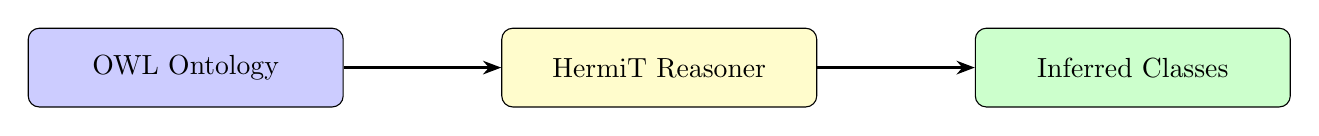
\begin{tikzpicture}[
    node distance=1cm,
    box/.style={rectangle, draw, rounded corners, minimum width=4cm, minimum height=1cm, text centered}
]
\node[box, fill=blue!20] (owl) {OWL Ontology};
\node[box, fill=yellow!20, right=2cm of owl] (reasoner) {HermiT Reasoner};
\node[box, fill=green!20, right=2cm of reasoner] (inferred) {Inferred Classes};

\draw[-{Stealth}, thick] (owl) -- (reasoner);
\draw[-{Stealth}, thick] (reasoner) -- (inferred);
\end{tikzpicture}

\subsection{Reasoning Results}

When the reasoner runs on hand-annotated individuals:

\begin{tabular}{|l|l|l|}
\hline
\textbf{Individual} & \textbf{Has Property?} & \textbf{Classified As} \\
\hline
Author\_HAND\_001 & careerStartYear = 2010 & ActiveAuthor \checkmark \\
Author\_HAND\_002 & No careerStartYear & AnonymousAuthor \checkmark \\
Article\_HAND\_001 & 1 author & SingleAuthorArticle \checkmark \\
Article\_HAND\_002 & 3 authors & MultiAuthorArticle \checkmark \\
\hline
\end{tabular}

\subsection{Python Code for Reasoning}

\begin{codebox}{reasoning.py}
\begin{lstlisting}[language=Python]
from owlready2 import *

onto = get_ontology("pkg2020_final.owl").load()

with onto:
    sync_reasoner(infer_property_values=True)

# Check consistency
print("Ontology is CONSISTENT")

# Check inferred classes
for a in onto.ActiveAuthor.instances():
    print(f"ActiveAuthor: {a.name}")
\end{lstlisting}
\end{codebox}

% ============== SECTION 8: WEB APPLICATION ==============
\newpage
\section{Web Application (Bonus)}

\subsection{Technology Stack}

\begin{tabular}{|l|l|}
\hline
\textbf{Component} & \textbf{Technology} \\
\hline
Backend & Flask (Python) \\
Frontend & HTML + D3.js \\
Database & GraphDB SPARQL Endpoint \\
Deployment & Heroku \\
SPARQL Client & SPARQLWrapper \\
\hline
\end{tabular}

\subsection{API Endpoints}

\begin{tabular}{|l|l|}
\hline
\textbf{Endpoint} & \textbf{Purpose} \\
\hline
\texttt{/} & Dashboard with statistics \\
\texttt{/sparql} & Raw SPARQL query interface \\
\texttt{/api/stats} & Graph statistics JSON \\
\texttt{/api/query} & Execute SPARQL query \\
\texttt{/api/competency-queries} & All 15 CQs \\
\texttt{/api/graph-data} & D3.js visualization data \\
\hline
\end{tabular}

\subsection{Visualization}

The web app includes an interactive D3.js force-directed graph showing:
\begin{itemize}
    \item All 23 ontology classes as nodes
    \item Object properties as edges
    \item Color-coded by category
    \item Interactive zoom and drag
\end{itemize}

% ============== SECTION 9: VIVA QUESTIONS ==============
\newpage
\section{Expected Viva Questions}

\subsection{Basic Questions}

\begin{enumerate}
    \item \textbf{What is T-Box vs A-Box?}\\
    T-Box = schema (classes, properties). A-Box = data (individuals).
    
    \item \textbf{What is a defined class?}\\
    Has necessary \& sufficient conditions. Reasoner classifies automatically.
    
    \item \textbf{What is a functional property?}\\
    Can have at most one value. Example: hasPrimaryAuthor.
    
    \item \textbf{What is SWRL?}\\
    Rule language for OWL. IF-THEN rules for inference.
    
    \item \textbf{How many triples in your graph?}\\
    2.2+ million triples.
\end{enumerate}

\subsection{Technical Questions}

\begin{enumerate}
    \item \textbf{Explain your enumeration class.}\\
    PublicationStatus = OneOf([Published, Preprint, Retracted, InReview])
    
    \item \textbf{Explain your intersection class.}\\
    ActiveAuthor = Author $\cap$ $\exists$careerStartYear.int
    
    \item \textbf{Explain your complement class.}\\
    AnonymousAuthor = Author $\cap$ $\neg$ActiveAuthor
    
    \item \textbf{How did you handle external linking?}\\
    DBpedia URIs for organizations, Wikidata for institutions.
    
    \item \textbf{What reasoner did you use?}\\
    HermiT via OWLReady2's sync\_reasoner().
\end{enumerate}

\subsection{Conceptual Questions}

\begin{enumerate}
    \item \textbf{Why convert CSV to RDF?}\\
    Semantic relationships, inference, linked data, SPARQL.
    
    \item \textbf{What is 5-star linked data?}\\
    1) Web, 2) Machine-readable, 3) Open format, 4) URIs, 5) Links to other data.
    
    \item \textbf{Benefits of knowledge graphs?}\\
    Complex queries, inference, integration, interoperability.
\end{enumerate}

% ============== SECTION 10: QUICK REFERENCE ==============
\newpage
\section{Quick Reference Card}

\begin{tcolorbox}[colback=primaryblue!5, colframe=primaryblue, title=Numbers to Remember]
\begin{tabular}{ll}
\textbf{Classes} & 23 (20+ required) \\
\textbf{Object Properties} & 14 (7+ required) \\
\textbf{Data Properties} & 17+ (7+ required) \\
\textbf{Triples} & 2.2 million \\
\textbf{Competency Questions} & 15 \\
\textbf{SWRL Rules} & 7 \\
\textbf{Hand-Annotated Individuals} & 13 \\
\end{tabular}
\end{tcolorbox}

\begin{tcolorbox}[colback=accentgreen!5, colframe=accentgreen, title=Key Files]
\begin{tabular}{ll}
\textbf{T-Box Only} & pkg2020\_tbox\_only.owl \\
\textbf{Hand Annotated} & pkg2020\_hand\_annotated.owl \\
\textbf{SWRL Rules} & pkg2020\_with\_swrl.owl \\
\textbf{Complete Data} & pkg2020\_final.owl / .ttl \\
\end{tabular}
\end{tcolorbox}

\begin{tcolorbox}[colback=warnorange!5, colframe=warnorange, title=Key Concepts]
\begin{tabular}{ll}
\textbf{Enumeration} & OneOf([...]) - fixed set of values \\
\textbf{Intersection} & $\sqcap$ or \& - AND condition \\
\textbf{Union} & $\sqcup$ or | - OR condition \\
\textbf{Complement} & $\neg$ or Not() - negation \\
\textbf{Functional} & Max 1 value allowed \\
\textbf{Inverse Functional} & Unique identifier \\
\end{tabular}
\end{tcolorbox}

\vfill
\begin{center}
\textcolor{primaryblue}{\Large\textbf{Good Luck with Your Viva! \faThumbsUp}}
\end{center}

\end{document}
